\section{Tradução automática neural - NMT}
Como apresentado na Seção \ref{chap:NMT}, a tradução automática neural é uma importante tarefa que tem como objetivo realizar a tradução de uma língua de origem para uma língua de destino por meio de sistemas computacionais, mais especificamente utilizando redes neurais artificiais. Essas redes buscam simular, de forma simplificada, o funcionamento do cérebro humano, permitindo a geração de traduções que se aproximem, o máximo possível, de traduções realizadas por humanos \cite{tan2020neural}.

As seções seguintes têm como objetivo apresentar os conceitos teóricos que fundamentam o estudo da arquitetura Transformer, proposta com o intuito de aprimorar a tarefa de tradução automática. Essa arquitetura introduz novos componentes e combina técnicas já existentes de forma mais eficiente. Como resultado, a arquitetura Transformer estabeleceu um novo estado da arte na tradução automática baseada em redes neurais artificiais \cite{DBLP:journals/corr/VaswaniSPUJGKP17}.

\section{Tokenização}

Tokenização, ou \textit{tokenization} em inglês, é uma etapa de pré-processamento fundamental no processamento de linguagem natural. Esse processo consiste em converter textos em unidades menores, como bytes, caracteres, subpalavras, palavras ou expressões de múltiplas palavras, denominadas \textit{tokens}. 

A Figura abaixo ilustra esse processo, no qual um texto é segmentado em tokens e, posteriormente, cada token é representado por valores numéricos que podem ser utilizados como entrada para redes neurais artificiais para realização da tradução entre linguas \cite{asgari2025morphbpemorphoawaretokenizerbridging}.

\begin{figure}[H]
    \centering
    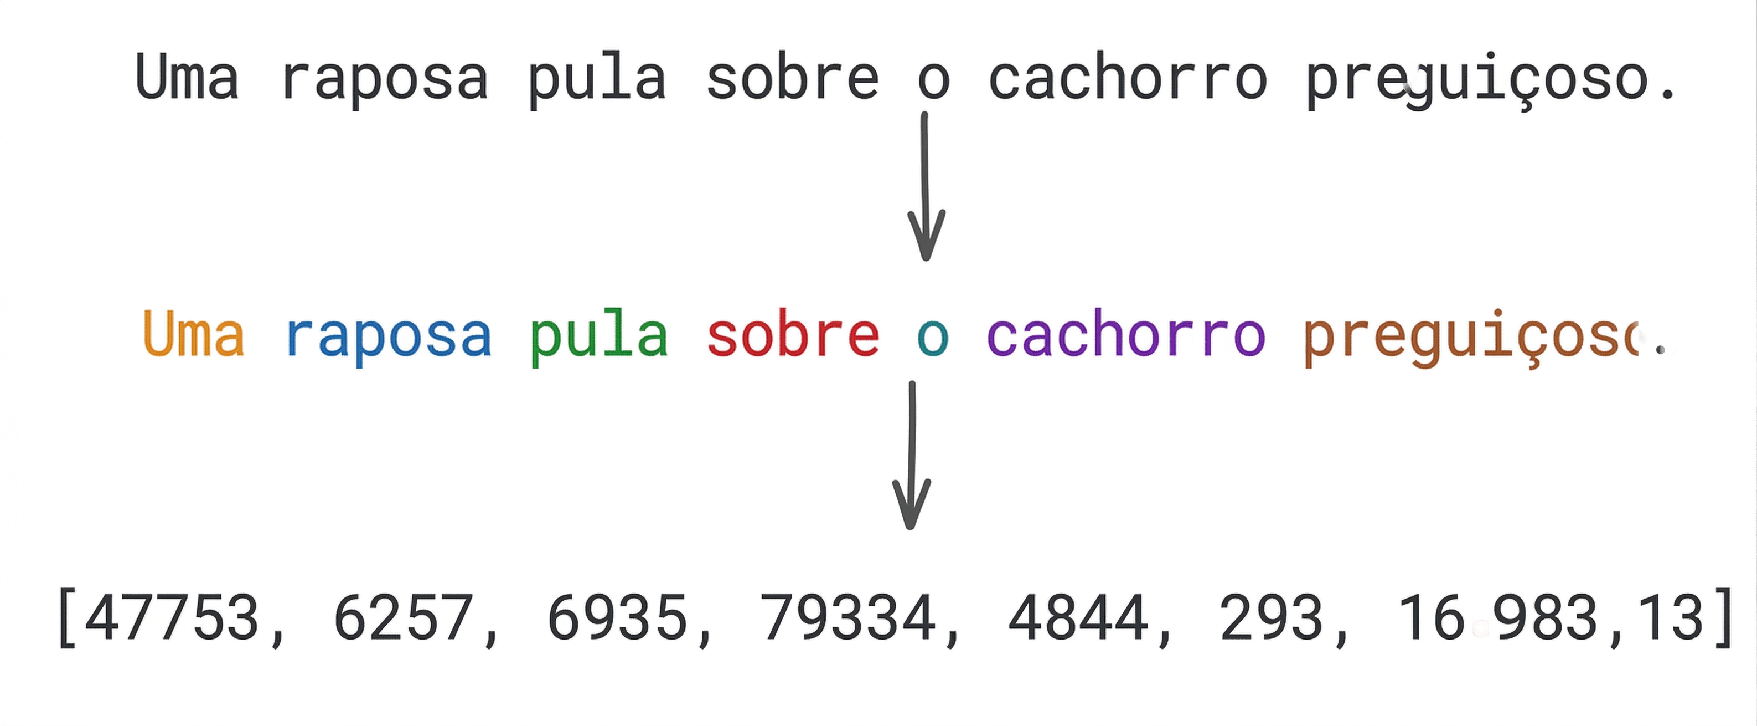
\includegraphics[width=.70\textwidth]{Imagens/tokenizer-referncial-teorico.pdf}

    \caption{\label{fig:tokenizer-rt}Tokenização de uma frase em português}

    \legend{Fonte: Criada pelo autor baseado na ferramenta \href{https://platform.openai.com/tokenizer}{openai tokenizer}}
\end{figure}



\section{Embedding}

\section{Modelo Sequence-to-Sequence}

\section{Função softmax}

\section{Mecanismo de Atenção}

\section{Arquitetura Transformer}
    \subsection{Visão Geral}
    \subsection{Codificador}
    \subsection{Decodificador}
    \subsection{Feed-Forward}
    \subsection{multi-head attention}
    \subsection{positional encoding}
    \subsection{paralelização}

\section{Modelos de Tradução Open Source}
    \subsection{MarianMT}
    \subsection{M2M}
    \subsection{NLLB}

\section{Métricas de Avaliação}
    \subsection{BLEU}
    \subsection{BERTScore}
    \subsection{chrF}

\section{Eficiência Computacional}